%% GENERATED FILE -- do not edit.
%% Written by scripts/manuscript/to_latex.py from manuscript/bmb_v4.md.
%% The markdown is the source; every number in it is recomputed by a script in
%% scripts/ and asserted by tests/.
%%
%% CLASS: Springer Nature sn-jnl, vendored at manuscript/springer/sn-jnl.cls
%% (LPPL). The option is sn-mathphys-ay -- AUTHOR-YEAR, which is what Bulletin of
%% Mathematical Biology uses and how the reference list below is written. The
%% Springer template ships with sn-mathphys-num uncommented; selecting it would
%% silently reformat the reference list into numbered style and break every
%% in-text citation, which are author-year throughout.
\documentclass[pdflatex,sn-mathphys-ay]{sn-jnl}

%% the class loads fontenc, geometry, hyperref, natbib, amsthm and others itself
\usepackage{amsmath,amssymb}
\usepackage{graphicx}
\usepackage[export]{adjustbox}
\usepackage{booktabs}
\usepackage{longtable}
\usepackage{array}
\usepackage{textcomp}
\usepackage{newunicodechar}
%% pandoc marks an uncaptioned longtable with \LTcaptype{none}; the caption
%% package then tries to step a counter of that name. Declaring it makes the
%% marker the no-op pandoc intends rather than a fatal error.
\newcounter{none}

\setlength{\emergencystretch}{3em}
\providecommand{\tightlist}{%
  \setlength{\itemsep}{0pt}\setlength{\parskip}{0pt}}

%% unicode that survives into prose, mapped from this document's own inventory
\newunicodechar{²}{$^{2}$}
\newunicodechar{×}{$\times$}
\newunicodechar{–}{--}
\newunicodechar{—}{---}
\newunicodechar{⁹}{$^{9}$}
\newunicodechar{⁻}{$^{-}$}
\newunicodechar{−}{$-$}
\renewcommand{\thefigure}{S\arabic{figure}}
\renewcommand{\topfraction}{0.92}
\renewcommand{\textfraction}{0.06}
\renewcommand{\floatpagefraction}{0.85}

\title[Collapse threshold for quality-control models]{An Exact Collapse Threshold for Conserved-Resource Models
       of Protein Quality Control}
\author*[1]{\fnm{Kiran} \sur{Boggavarapu}}\email{kiran@mcneese.edu}
\affil*[1]{\orgdiv{Department of Chemistry and Physics}, \orgname{McNeese State University}, \orgaddress{\city{Lake Charles}, \state{LA}, \postcode{70609}, \country{USA}}}

\abstract{Supplementary material accompanying the paper above. Every number in the caption is recomputed by the script named in it and asserted by the accompanying test suite.}

\begin{document}
\maketitle

\begin{figure}[htbp]
\centering
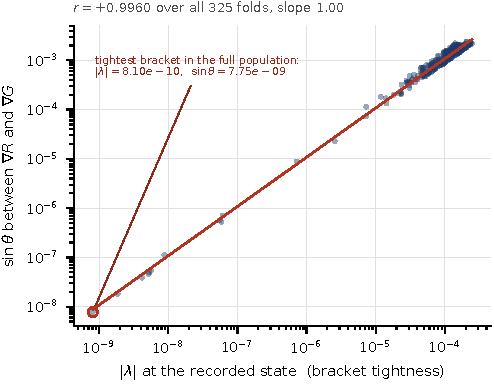
\includegraphics[max width=\linewidth]{../figures/figS1.pdf}
\caption{The parallelism residual is bracket tolerance, not failure of the identity. Over all 325 folds of the load grid, $\sin \theta$ between $\nabla R$ and $\nabla G$ tracks the leading eigenvalue recorded at the same state across five decades, with a log–log correlation of +0.9960 and a slope of 1.00 — the residual is \emph{proportional} to how loosely the state is bracketed, which is what bracket tolerance means and what a failing identity would not produce. The circled point is the tightest bracket in the population, $|\lambda | = 8.10\times 10^{-10}$ with $\sin \theta = 7.75\times 10^{-9}$. Normalisation, reported here rather than given a panel of its own: on these same 325 states the max-normalised residual correlates with $|\lambda |$ at −0.835 and reaches 1.54×10⁻², while the gradient-normalised residual used throughout correlates at +0.041 and reaches 1.29×10⁻⁹. The first degrades as the bracket tightens on the object it is meant to verify, because both $\det J$ and the cross product vanish at a saddle-node and their ratio is 0/0 there; the second does not. Every number in this caption is recomputed by \texttt{scripts/\allowbreak figures/\allowbreak fig\_identity.py:captionNumbers} and asserted by the test suite.}
\label{fig:figS1}
\end{figure}

\begin{center}\rule{0.5\linewidth}{0.5pt}\end{center}

\end{document}
